\documentclass[12pt, a4paper]{article}
\usepackage{geometry}
\geometry{margin=2.5cm}
\usepackage{graphicx}
\usepackage{amsmath}
\usepackage{enumitem}
\usepackage[utf8]{inputenc}
\usepackage[french]{babel}
\usepackage{listings}
\usepackage{xcolor}
\usepackage[hidelinks]{hyperref}

\title{SAÉ 3.01 Rapport de probas/stats}
\author{Jules CHIRON, Matis RODIER, Thomas GODINEAU | INF2 FI A}
\date{12 janvier 2024}

\NewDocumentCommand{\codeword}{v}{%
\texttt{\textcolor{blue}{#1}}%
}

\usepackage[T1]{fontenc}
\begin{document}
\maketitle

\begin{figure}[h]
    
\includegraphics[width=0.6\textwidth]{../annexes/logo_uvsq}
\end{figure}

\tableofcontents{}

\section*{Introduction}
\addcontentsline{toc}{section}{Introduction}

Le but de cette SAÉ est de réaliser une \textbf{application web} de ticketing en PHP.\@
Chaque utilisateur de cette plateforme peut créer un compte, se connecter et créer un ticket qui sera pris en charge par un technicien.
Dans la partie probas/stats de ce projet, nous avons réalisé une page web qui permet de visualiser des statistiques sur les tickets et les connexions
en utilisant le module \textbf{Shiny} de \textbf{R}.
\bigskip

La \textbf{première partie} de ce rapport contient une présentation du module \textbf{Shiny}.
La \textbf{deuxième partie} contient une présentation de notre code et de son contenu.
Enfin, la \textbf{troisième partie} contient une présentation du déploiement de notre application.

\section{Présentation}

Le langage \textbf{R} est un langage de programmation apparu en 1993.
Ce langage a pour but de réaliser des statistiques et des graphiques en étudiant des données.
\bigskip

Le module \textbf{Shiny} est un module de \textbf{R} qui a commencé à être développé en 2012.
Ce  module permet de créer des applications web en \textbf{R}.
Il permet de créer des pages web qui contiennent des graphiques et des statistiques
et qui disposent d'une interface graphique permettant aux utilisateurs de choisir les paramètres des données qu'ils souhaitent étudier.
\bigskip

\noindent Le module \textbf{Shiny} peut être installé directement depuis la console \textbf{R} avec la commande suivante:
\begin{center}
    \codeword{install.packages("shiny")}
\end{center}

\section{Notre page}

\noindent Notre page Shiny contient 3 principaux éléments:
\begin{itemize}
    \item L'interface utilisateur (\textit{ui})
    \item La partie serveur (fonction) (\textit{server})
    \item ShinyApp (fonction)
\end{itemize}
\bigskip
\textit{Le code de notre page ainsi que les fichiers csv utilisés se trouvent dans le dossier \textbf{src/} fourni avec ce rapport.}

\subsection*{Déroulement du programme}
\addcontentsline{toc}{subsection}{Déroulement du programme}\label{subsec:deroulement}

Nous commençons notre programme en chargeant la bibliothèque \textbf{shiny} avec la fonction \codeword{library(shiny)}.
Puis on règle le port par défaut de l'application pour qu'elle soit toujours accessible sur le même port (\textit{port 3000})
avec la fonction \codeword{options(shiny.port = 3000)}.
\bigskip

Nous ajoutons ensuite les éléments \textit{ui} et \textit{server}.
Puis nous lançons l'application avec la fonction \codeword{shinyApp(ui, server)}.

\subsection*{Interface utilisateur}
\addcontentsline{toc}{subsection}{Interface utilisateur}

\noindent \textit{La Figure~\ref{fig:shiny_ui} représente la partie \textbf{ui} de notre page.}
\bigskip

L'élément \textbf{ui} correspond à une \textbf{fluidPage} qui contient l'interface utilisateur de notre application.
Notre \textbf{fluidPage} contient 3 éléments:
\begin{itemize}
    \item Un \textbf{titlePanel}: titre
    \item Deux \textbf{sidebarLayout}: choix des \textit{paramètres} et représentation des \textit{résultats}
\end{itemize}
L'élément \textbf{titlePanel} permet de mettre un titre à notre page, on l'a appelée ici `Statistiques'.
Nos \textbf{sidebarLayout} contiennent chacun un \textbf{sidebarPanel} et un \textbf{mainPanel}.
\bigskip

Le premier \textbf{sidebarLayout} sert à choisir les paramètres pour la première statistique (le pourcentage de tickets selon leur statut).
Son \textbf{sidebarPanel} contient un \textbf{titlePanel} permettant de donner un titre au panel, ainsi que deux \textbf{inputs} (\textit{élément de choix}):
\begin{itemize}
    \item Le premier input est un \textit{selectInput} qui permet de choisir entre les différents statuts de ticket
    (open (\textit{ouvert}), in\_progress (\textit{en cours}), closed (\textit{fermé}))
    \item Le deuxième input est un \textit{numericInput} qui permet de choisir le nombre de tickets à étudier (entre 1 et 40)
\end{itemize}
Son \textbf{mainPanel} contient deux outputs (\textit{sorties}):
\begin{itemize}
    \item Le premier est de type \textit{verbatimTextOutput} > la sortie sera sous forme de texte
    \item Le deuxième est de type \textit{plotOutput} > la sortie sera un graphique
\end{itemize}
\bigskip

Le deuxième \textbf{sidebarLayout} sert aux choix des paramètres de la seconde statistique (le pourcentage de connexions réussies).
Son \textbf{sidebarPanel} contient un \textbf{titlePanel} et un seul input:
\begin{itemize}
    \item L'input est un \textit{numericInput}  qui permet de choisir le nombre de connexions que l'on souhaite étudier.
\end{itemize}
Son \textbf{mainPanel} contient deux \textit{outputs}:
\begin{itemize}
    \item Les deux sont de type \textit{plotOutput} > il y aura donc deux graphiques.
\end{itemize}

\subsection*{Partie serveur}
\addcontentsline{toc}{subsection}{Partie serveur}

\noindent \textit{La Figure~\ref{fig:shiny_server} représente différents outputs définis dans la partie \textbf{serveur} de notre programme.}
\bigskip

Notre fonction \textbf{server} commence par récupérer les données des fichiers csv (\textit{tickets.csv} et \textit{connexions.csv}).
Nous avons créé ces deux fichiers en s'inspirant des données présentes dans la base de données de l'application.

\noindent Nous paramétrons ensuite les représentations de nos différents \textit{outputs}.
Ils sont listés dans l'ordre décrit dans la partie précédente:

\begin{itemize}
    \item Le premier est une zone de texte contenant le pourcentage de ticket selon le type choisis dans le \textit{selectInput}.
    \item Le deuxième est un graphique en camembert dont chaque partie représente le pourcentage de chaque statut de ticket.
    \item Le troisième est encore un graphique en camembert dont chaque partie représente le pourcentage de connexions réussies ou échouées.
    \item Le quatrième graphique est la représentation du pourcentage de connexions réussies sous forme de points.
\end{itemize}

\section{Déploiement}

Nous avons d'abord souhaité héberger notre serveur Shiny sur le \textbf{Raspberry Pi} fourni pour la SAÉ.
Cependant, il s'est avéré impossible de lancer une application Shiny sur ce serveur.
Nous avons essayé d'installer \textbf{R} et le \textbf{module Shiny} depuis les dépôts officiels mais nous avions une \textit{erreur de bus}.
Nous avons donc installé \textbf{R} par compilation depuis les sources.
Cependant, nous avions toujours une erreur lors du lancement de l'application.
Nous ne pouvions même pas lancer les applications de test (\textit{01\_hello, 02\_text \ldots}) fournies \textbf{par Shiny}.
\bigskip

Finalement, nous avons décidé de déployer notre application Shiny sur un serveur \textbf{shinyApps.io}.
Ce site est un site officiel de \textbf{Shiny} qui permet d'héberger des applications Shiny.
Nous avons créé un compte gratuit qui permet d'héberger jusqu'à 5 applications.
Cependant, une application ne peut être \textit{active} (chargée sur un navigateur) que 25 heures par mois.
Étant donné que cette page ne sert que dans ce projet (il est très peu probable qu'elle soit chargée très longtemps),
nous avons choisi cette solution.
\bigskip

\noindent Notre application est donc accessible depuis l'adresse suivante:
\begin{center}
    \url{https://Boucanier.shinyapps.io/proba}
\end{center}

\noindent Nous avons intégré notre application dans un \textbf{iframe} sur notre site web.
Elle est consultable depuis la page \textbf{Statistiques} (\textit{stats.php}) de la plateforme,
accessible pour \textbf{l'administrateur système}.

\bigskip
Si nous avions hébergé notre application sur le Raspberry Pi,
nous aurions pu l'intégrer en mettant un \textbf{iframe} avec l'adresse \textbf{localhost\string:3000} (cf~\ref{subsec:deroulement}).

\newpage

\section{Annexes}
\bigskip
\begin{figure}[ht]
    \centering
    \frame{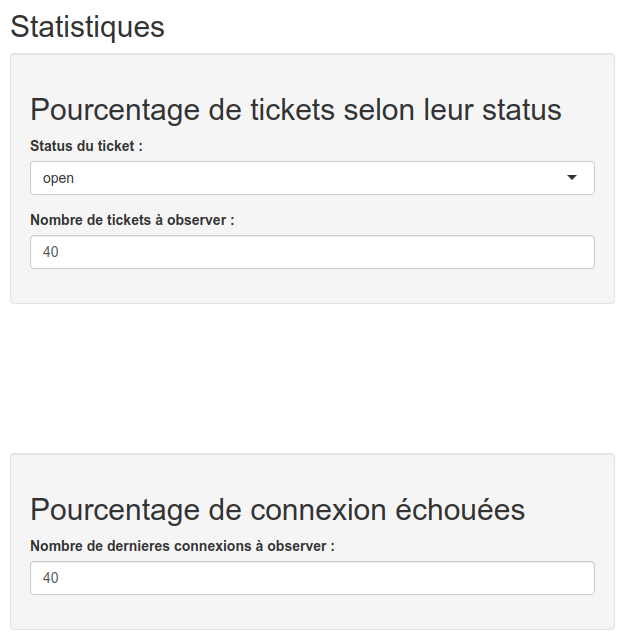
\includegraphics[width=0.9\textwidth]{../annexes/shiny_ui.png}}
    \caption{Partie Interface Utilisateur de notre page}\label{fig:shiny_ui}
\end{figure}
\begin{figure}[ht]
    \centering
    \frame{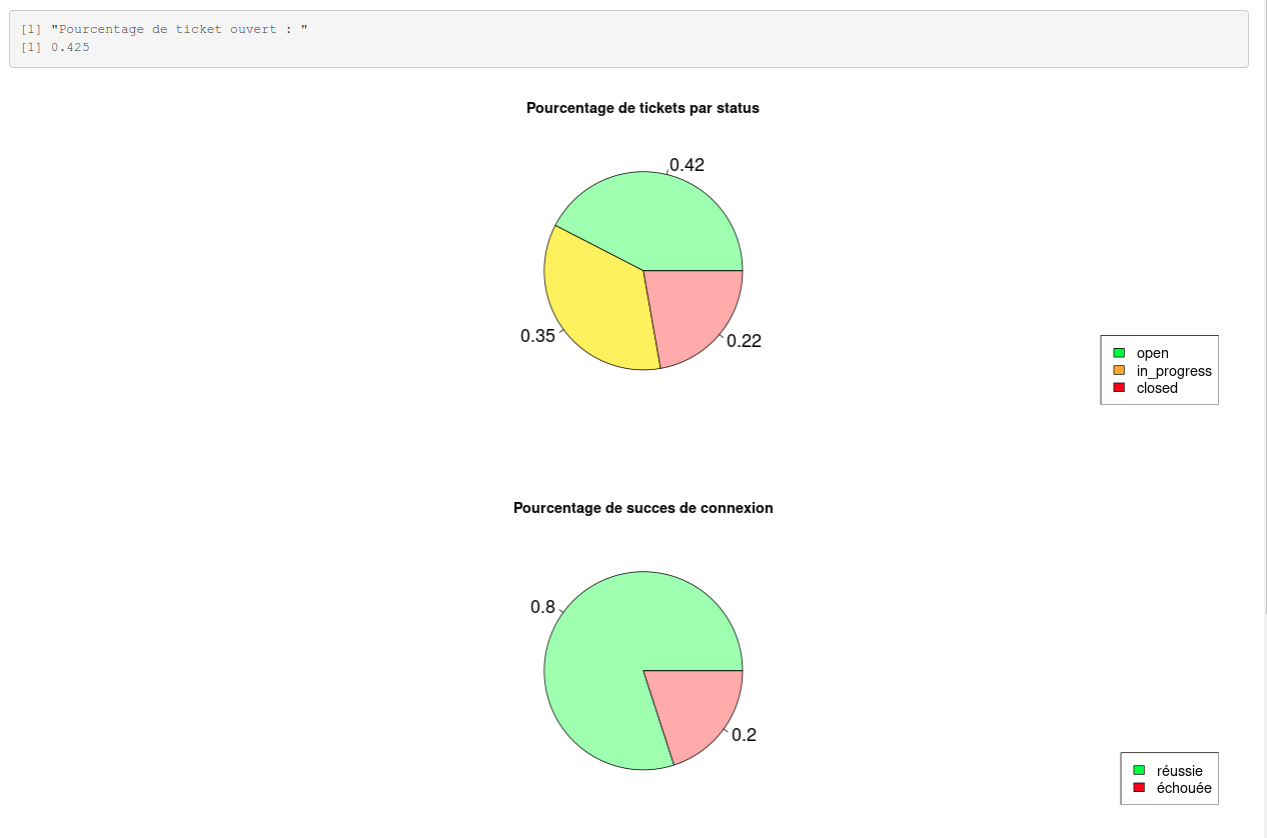
\includegraphics[width=0.9\textwidth]{../annexes/shiny_server.png}}
    \caption{Différents \textit{outputs} de notre application}\label{fig:shiny_server}
\end{figure}

\end{document}